%%%%%%%%%%%%%%%%%%%%%%%%%%%%%%%%%%%%%%%%%%%%%%%%%%%%%%%%%%%%%%%%%%%%%%%%%%%%%%%%
%%%%%%%%%%%%%%%%%%%%%%%%%%%%%%%%%%%%%%%%%%%%%%%%%%%%%%%%%%%%%%%%%%%%%%%%%%%%%%%%
%%                                                                            %%
%% opintnaytepohja.tex versio 3.01 (2017/10/06)                               %%
%% Opinnäytepohja käytettäväksi aaltothesis.sty (versio 3.01) -tyylitiedoston %%
%% kanssa.                                                                    %%
%% Toimiakseen paketti tarvitsee pdfx.sty v. 1.5.84 (2017/05/18) tai uudempi. %%
%% The LaTeX template file to be used with the aaltothesis.sty (version 3.0)  %%
%% style file.                                                                %%
%% This package requires pdfx.sty v. 1.5.84 (2017/05/18) or newer.            %%
%%                                                                            %%
%% This is licensed under the terms of the MIT license below.                 %%
%%                                                                            %%
%% Copyright 2017, by Luis R.J. Costa, luis.costa@aalto.fi,                   %%
%% Copyright 2017 documentation in Finnish in the template by Perttu Puska,   %%
%% perttu.puska@aalto.fi                                                      %%
%% Copyright Swedish translations 2014 by Elisabeth Nyberg,                   %%
%% elisabeth.nyberg@aalto.fi and Henrik Wagllén, henrik.wallen@aalto.fi       %%
%%                                                                            %%
%% Permission is hereby granted, free of charge, to any person obtaining a    %%
%% copy of this software and associated documentation files (the "Software"), %%
%% to deal in the Software without restriction, including without limitation  %%
%% the rights to use, copy, modify, merge, publish, distribute, sublicense,   %%
%% and/or sell copies of the Software, and to permit persons to whom the      %%
%% Software is furnished to do so, subject to the following conditions:       %%
%% The above copyright notice and this permission notice shall be included in %%
%% all copies or substantial portions of the Software.                        %%
%% THE SOFTWARE IS PROVIDED "AS IS", WITHOUT WARRANTY OF ANY KIND, EXPRESS OR %%
%% IMPLIED, INCLUDING BUT NOT LIMITED TO THE WARRANTIES OF MERCHANTABILITY,   %%
%% FITNESS FOR A PARTICULAR PURPOSE AND NONINFRINGEMENT. IN NO EVENT SHALL    %%
%% THE AUTHORS OR COPYRIGHT HOLDERS BE LIABLE FOR ANY CLAIM, DAMAGES OR OTHER %%
%% LIABILITY, WHETHER IN AN ACTION OF CONTRACT, TORT OR OTHERWISE, ARISING    %%
%% FROM, OUT OF OR IN CONNECTION WITH THE SOFTWARE OR THE USE OR OTHER        %%
%% DEALINGS IN THE SOFTWARE.                                                  %%
%%                                                                            %%
%%                                                                            %%
%%%%%%%%%%%%%%%%%%%%%%%%%%%%%%%%%%%%%%%%%%%%%%%%%%%%%%%%%%%%%%%%%%%%%%%%%%%%%%%%
%%                                                                            %%
%%                                                                            %%
%% Esimerkki opinnäytteen tekemisestä LaTeX:lla                               %%
%% Alkuperäinen versio ja kehitystyö Luis Costa, muutokset Perttu Puska       %%
%% Ruotsinkielen tuki lisätty 15092014                                        %%
%% PDF/A-tuki lisätty 15092017                                                %%
%%                                                                            %%
%% Tähän esimerkkiin kuuluu tiedostot                                         %%
%%         opinnaytepohja.tex (versio 3.01)                                   %%
%%         thesistemplate.tex (versio 3.01) (for text in English)             %%
%%         aaltothesis.cls (versio 3.01)                                      %%
%%         kuva1.eps                                                          %%
%%         kuva2.eps                                                          %%
%%         kuva1.pdf                                                          %%
%%         kuva2.pdf                                                          %%
%%                                                                            %%
%%                                                                            %%
%% Kääntäminen Linuxissa joko                                                 %%
%% latex:                                                                     %%
%%             $ latex opinnaytepohja                                         %%
%%             $ latex opinnaytepohja                                         %%
%%                                                                            %%
%%   Tuloksena on tiedosto opinnayte.dvi, joka muutetaan ps-muotoon           %%
%%   seuraavasti                                                              %%
%%                                                                            %%
%%             $ dvips opinnaytepohja -o                                      %%
%%                                                                            %%
%%   ja edelleen pdf-muotoon seuraavasti                                      %%
%%                                                                            %%
%%             $ ps2pdf opinnaytepohja.ps                                     %%
%%                                                                            %%
%% Tai                                                                        %%
%% pdflatex:                                                                  %%
%%             $ pdflatex opinnaytepohja                                      %%
%%             $ pdflatex opinnaytepohja                                      %%
%%                                                                            %%
%%   Tuloksena on tiedosto opinnaytepohja.pdf                                 %%
%%                                                                            %%
%% Selittävät kommentit on tässä esimerkissä varustettu %%-merkeillä ja       %%
%% muutokset, joita käyttäjä voi tehdä, on varustettu %-merkeillä             %%
%%                                                                            %%
%%%%%%%%%%%%%%%%%%%%%%%%%%%%%%%%%%%%%%%%%%%%%%%%%%%%%%%%%%%%%%%%%%%%%%%%%%%%%%%%
%%%%%%%%%%%%%%%%%%%%%%%%%%%%%%%%%%%%%%%%%%%%%%%%%%%%%%%%%%%%%%%%%%%%%%%%%%%%%%%%

%% Käytä yksi näistä:
%% ensimmäinen, jos käytät pdflatexia, joka kääntää tekstin suoraan
%% pdf-tiedostoksi (kuvat on oltava jpg-, png- tai pdf-tiedostoina. Kun teet
%% PDF/A-muotoista pdf-dokumenttia älä käytä PDF/A-muotoista tiedostoa kuvissa.)
%% ja haluat tulostaa opinnäytteesi
%% toinen, jos haluat verkkossa julkaistava PDF/A-muotoista tiedostoa
%% kolmas jos haluat tuottaa ps-tiedostoa (käytä eps-formaattia kuville, älä
%% käytä ps-muotoisia kuvia!)
%%
%\documentclass[finnish, 12pt, a4paper, elec, utf8, pdfa]{aaltothesis}
\documentclass[finnish, 12pt, a4paper, elec, utf8, pdfa, online]{aaltothesis}
%\documentclass[finnish, 12pt, a4paper, dvips]{aaltothesis}

%% Kirjoita y.o. \documentclass optioiksi
%% korkeakoulusi näistä: arts, biz, chem, elec, eng, sci
%% editorisi käyttämä merkkikoodaustapa: utf8, latin1
%% opinnäytetyön kieli: finnish, english, swedish
%% tee arkistointikelpoista PDF/A-1b pdf-tiedosto: pdfa
%% verkkoon menevä symmetrinen taitto ja hypertekstin väri on sininen: online
%%                        (ei optiota on oletusarvo, tuloksena leveä marginaali
%%                         sivun sidonta puolella ja musta hyperteksti)
%% kaksipuolinen tulostus: twoside (oletusarvo on yksipuolinen tulostus)
%%

%% Käytä yksi näistä, jos kirjoitat englanniksi. Katso englanninokset
%% tiedostosta thesistemplate.tex.
%\documentclass[english, 12pt, a4paper, elec, utf8, pdfa]{aaltothesis}
%\documentclass[english, 12pt, a4paper, elec, utf8, pdfa, online]{aaltothesis}
%\documentclass[english,12pt, a4paper, dvips]{aaltothesis}

\usepackage{graphicx}

%% Matematiikan fontteja, symboleja ja muotoiluja lisää, näitä tarvitaan usein
\usepackage{amsfonts,amssymb,amsbsy}


%% Korjaa vastaamaan korkeakouluasi, jos automaattisesti asetettu nimi on
%% virheellinen
%%
%% Change the school field to specify your school if the automatically
%% set name is wrong
% \university{aalto-yliopisto}
% \school{Sähkötekniikan korkeakoulu}

%% Korjaa seuraava vastaamaan koulutusohjelmaasi
%%
\degreeprogram{Sähkötekniikan kandidaattiohjelma}
%%

%% Pääaineesi
\major{Automaatio ja systeemitekniikka}

%% Pääainekoodi
%%
%%\code{}
%%

%% Valitse yksi näistä kolmesta
%%
\univdegree{BSc}
%\univdegree{MSc}
%\univdegree{Lic}
%%

%% Oma nimi
%%
\thesisauthor{Joni Airaksinen}
%%

%% Opinnäytteen otsikko tulee tähän ja mahdollisesti uudelleen englannin- tai
%% ruostinkielisen abstraktin yhteydessä. Älä tavuta otsikkoa ja vältä liian
%% pitkää otsikkotekstiä. Jos latex ryhmittelee otsikon huonosti, voit joutua
%% pakottamaan rivinvaihdon \\ kontrollimerkillä.
%% Tällöin...
%% Muista että otsikkoja ei tavuteta!
%% Jos otsikossa on ja-sana, se ei jää rivin viimeiseksi sanaksi vaan aloittaa
%% uuden rivin.
%% Anna ostikko uudelleen ilman rivinvaihtomerkkiä optionaalisena argumenttina
%% hakasuluissa. Näin tehdään, koska otsikko on osaa pdf/a-tiedostossa olevaa
%% metadataa, ja metadatassa ei saa olla rivinvaihtomerkkiä.
%%
\thesistitle{Semanttinen internet}
%\thesistitle[Opinnäytteen otsikko]{Opinnäyteen\\ otsikko}
%%

\place{Espoo}

%% Kandidaatintyön päivämäärä on sen esityspäivämäärä!
%%
\date{23.4.2018}
%%

%% Kandidaattiseminaarin vastuuopettaja tai diplomityön valvoja.
%% Huomaa tittelissä "\" -merkki pisteen jälkeen, ennen välilyöntiä ja
%% seuraavaa merkkijonoa.
%% Näin tehdään, koska kyseessä ei ole lauseen loppu, jonka jälkeen tulee
%% hieman pidempi väli vaan halutaan tavallinen väli.
%%
\supervisor{TkT.\ Pekka Forsman}
%%

%% Kandidaatintyön ohjaaja(t) tai diplomityön ohjaaja(t). Ohjaajia saa
%% olla korkeintaan kaksi.
%%
%\advisor{Prof.\ Pirjo Professori}
\advisor{TkL Pekka Aarnio}
%\advisor{DI Tina Tutkija}
%%

%% Aaltologo: syntaksi:
%% \uselogo{aaltoRed|aaltoBlue|aaltoYellow|aaltoGray|aaltoGrayScale}{?|!|''}
%% Logon kieli on sama kuin dokumentin kieli
%%
\uselogo{aaltoRed}{''}
%%

%% Suomenkielinen tiivistelmä:
%% Kaikki tiivistelmässä tarvittava tieto (nimesi, työnnimi, jne.) käytetään
%% niin kuin se on yllä määritelty.
%% Tiivistelmän avainsanat:
%% Huom! Avainsanat erotetaan toisistaan \spc -makrolla
%%
\keywords{Semanttinen internet\spc RDF}

%% Tiivistelmän tekstiosa. Tämä teksti sisältyy pdf-tiedoston metadataa ja tulee
%% myös tiivistelmälomakkeeseen.
%%
\thesisabstract{
Semanttinen internet mahdollistaa tiedon tehokkaan jakamisen ja hyödyntämisen. Kaikki saatavilla oleva tieto ei kuitenkaan ole semanttista. Tämä johtuu siitä, että semanttisen tiedon luominen vaatii ylimääräistä vaivannäköä ja resursseja. Toinen hidaste semanttisen tiedon synnylle on ihmisten tietämättömyys asiasta. Kovinkaan moni ihminen ei pysty määrittelemään termiä: semanttinen internet, vaikka
semanttinen internet kuuluukin hyvin monen ihmisen arkeen. Pelkästään yksittäinen Google haku tuo käyttäjälle esiin linkittynyttä tietoa, joka on mahdollisesti muodostettu hyödyntäen semanttisen verkon työkaluja. Tutkielmassa selvitetään semanttisen verkon luomiseen vaadittavat vähimmäistyökalut. Tutkielman tarkoituksena on selkeyttää semanttisen internetin merkitystä ja tutustuttaa lukija linkittyneen tiedon luomiseen. Lisäksi tutkielmassa yritetään tuoda ilmi semanttisen internetin tuomia hyötyjä ja hyviä käyttökohteita.
}

%% Tekijänoikeusteksti. Tekijänoikeus on tekijällä riippumatta siitä onko
%% copyright -merkintä näkyvissä vai ei. Halutessasi voit jakaa työsi Creative
%% Commons -lisensillä (katso creativecommons.org), jolloin lisenssitekstin on
%% oltava näkyvissä. Kirjoita tähän haluamasi tekijänoikeustekstin. Se kirjautuu
%% myös pdf-tiedoston metadataan.
%% Syntaksi:
%% \copyrigthtext{metadatateksti}{sivulle näkyviin tuleva teksti}
%%
%% A.o. metadataan menevässä tekstissä on käytettävä \noexpand -makroa ennen
%% \copyright -erikoismerkkiä ja makrot (tässä \copyright ja \year) on erotettava
%% seuraavasta tekstistä \ -merkillä (välilyöntimerkki). \copyrighttext-makron
%% argumentissa olevat makrot automaattisesti hakevat vuosiluvun ja tekijän nimi.
%% (Huom! \ThesisAuthor on aaltothesis.cls -tyylitiedoston sisäinen makro).
%% Toki saman tekstin olisi voinut kirjoittaa yksinkertaisesti näin:
%% \copyrighttext{Copyright \noexpand\copyright\ 2017 Teemu Teekkari}
%% {Copyright \copyright{} 2017 Teemu Teekkari}
%%
\copyrighttext{Copyright \noexpand\copyright\ \number\year\ \ThesisAuthor}
{Copyright \copyright{} \number\year{} \ThesisAuthor}

%% Voit estää LaTeXia kirjoittamasta xmpdata-tiedostoon (sisältää pdf-tiedostoon
%% kirjoitettavaa metadataa) asettamalla writexmpdatafile lipun arvoksi 'false'.
%% Tämä mahdollistaa sen, että voit kirjoittaa metadataa suoraan oikeassa
%% muodossa tiedostoon opinnaytepohja.xmpdata.
%%
%\setboolean{writexmpdatafile}{false}

%%-------------------------------------------------------------------------------
%% OMAT ASETUKSET:
%% Aseta tyjä rivi kappaleiden väliin
\usepackage[parfill]{parskip}

%% Vaihdetaan sisällysluettelon väri mustaksi
\usepackage{hyperref}% http://ctan.org/pkg/hyperref
\hypersetup{
  colorlinks = true,
  linkcolor  = black
}

%% Seuraavalla päästään eroon turhista \hbox warningeista:
\usepackage{etoolbox}
\apptocmd{\sloppy}{\hbadness 10000\relax}{}{}

\usepackage{listings}
\lstdefinestyle{codeblock}{
  language=XML,
  numbers=left,
  numbersep=0.75em,
  frame=single,
  framesep=\fboxsep,
  framerule=\fboxrule,
  rulecolor=\color{black},
  xleftmargin=0.60cm,
  xrightmargin=\dimexpr\fboxsep+\fboxrule\relax,
  breaklines=true,
  tabsize=2,
  columns=flexible,
}

%% Salli svg kuvat
\usepackage{svg}
\usepackage{amsmath}
%%-------------------------------------------------------------------------------


%% Kirjoitelman alku
\begin{document}

%% Tehdään kansilehti
%%
\makecoverpage

%% Tehdään tekijänoikeusteksti näkyväksi.
%% Halutessasi voit jättää tekijänoikeustekstin pois luettavasta pdf-tiedostosta.
%% Tämä voi tuntua hyvältä ajatukselta paperille tulostetulla versiossa eteenkin,
%% jos sivun ainoa teksti on "Copyright (c) vvvv Teemu Teekkari". Suositus on
%% kuitenkin jättää teksti näkyviin.
%%
\makecopyrightpage

%% Suomenkielinen tiivistelmä
%% Kaikki tiivistelmässä tarvittava tieto (nimesi, työnnimi, jne.) käytetään
%% niin kuin se on yllä määritelty.
%%
%% Tiivistelmän tekstiosa
%%
\begin{abstractpage}[finnish]
Semanttinen internet mahdollistaa tiedon tehokkaan hyödyntämisen ja levittämisen. Hyödyistään huolimatta, semanttinen internet on monille tuntematon käsite ja siten vähän ymmärretty asiakokonaisuus. Tutkielma pyrkii tiivistämään semanttisen internetin pääkohdat lyhyeen ja selkeään esitysmuotoon. Lukijan ei oleteta entuudestaan tietävän aiheesta juuri mitään. Jotta semanttisesta internetistä kertominen olisi mielekästä, niin tutkielman alussa määritellään termin merkitys. Tämän jälkeen esitellään semanttisen internetin keskeisimpiä tekniikoita, kuten esimerkiksi: RDF(S), OWL ja SPARQL. Lopuksi esitellään sovelluksia, jotka hyödyntävät semanttista internetiä.
\end{abstractpage}

%% \thesisabstract -makrossa kirjoitettu teksti on tallennettu \abstractext
%% -makrosa jolloin voit siirtää metadataan menevä teksti sellaisenaan näin:
%%
%\begin{abstractpage}[finnish]
%	\abstracttext{}
%\end{abstractpage}

%% Pakotetaan uusi sivu varmuuden vuoksi, jotta mahdollinen suomenkielinen ja
%% englanninkielinen tiivistelmä eivät tule vahingossakaan samalle sivulle
%%
\newpage





%% Esipuhe
%%
\mysection{Esipuhe}
tmp

\vspace{5cm}
Otaniemi, xx.yy.2018

\vspace{5mm}
{\hfill Joni Airaksinen \hspace{1cm}}

%% Pakotetaan varmuuden vuoksi esipuheen jälkeinen osa
%% alkamaan uudelta sivulta
\newpage


%% Sisällysluettelo
%%
\thesistableofcontents


%% Symbolit ja lyhenteet
%%
\mysection{Lyhenteet}

\subsection*{Semanttiseen internet}
\begin{tabular}{ll}
HTTP         & Hypertext Transfer Protocol \\
OWL          & Web Ontology Language \\
RDF          & Resource Description Framework \\
RDFS         & Resource Description Framework Schema\\
SPARQL       & SPARQL Protocol and RDF Query Language \\
Turtle       & Terse RDF Triple Language \\
WWW          & World Wide Web \\
W3C          & World Wide Web Consortium \\
XML          & Extensible Markup Language \\
XMP          & Extensible Metadata Platform \\

URI          & Uniform Resource Identifier \\
URL          & Uniform Resource Locator \\
\end{tabular}

\subsection*{Esimerkit}
\begin{tabular}{ll}
Cpu          & Central Processing Unit \\
Gpu          & Graphics Processing Unit \\
Hdd          & Hard Disk Drive \\
Psu          & Power Supply Unit \\
Ram          & Random Access Memory \\
Ssd          & Solid State Drive \\
\end{tabular}

%% \clearpage on melkein samanlainen kuin newpage, mutta
%% flushaa myös LaTeX:n floatit
%%
\cleardoublepage

%% MEMO:
%% Tietämyksen esittämiskieli
%%
%%
%% Selitä metadata?
%%
%% Internet sana isolla, koska se korostaa sanaa. Internet sana on lauseissa
%% yleensä hyvin merkityksellinen, joten on hyvä jos se erottuu muiden seasta.
%%
%% "This classical layer cake was a major driver in the agenda of the Semantic Web,
%%ut is now quite outdated" (PRIMER, s.18) - älä esittele kakkumallia?

%%===============================================================================
%% Leipäteksti alkaa
\section{Johdanto}

%% Ensimmäinen sivu tyhjäksi
\thispagestyle{empty}
Internet on luotu tiedon jakamista varten. Aluksi internetin avulla jaettiin ihmisten kirjoittamia tekstidokumentteja kuten esimerkiksi tutkimustuloksia. Dokumenteissa esitetty tieto oli kirjoitettu muita ihmisiä varten. Tietokoneet pystyivät kuitenkin seulomaan sanoja, ja näin hylkäämään epämääräisiä dokumentteja, mutta mihinkään edistyksellisempään ne eivät kyenneet \cite{WWW}. Internetin kehittäjä Tim Berners-Lee halusi hyödyntää tietokoneita internetin yhteydessä entistäkin enemmän, joten hän alkoi kehittämään internetin jatkeeksi luonnehdiltua semanttista internetiä (engl. Semantic Web) \cite{Berners_visio}.

Termillä semanttinen internet viitataan internettiin, jonka sisältö on luotu käyttäen standardoituja tekniikoita, jotka mahdollistavat loogisten päätelmien tekemisen sekä ihmiselle että tietokoneelle. \cite{Berners_visio}. Semanttinen internet pyrkii siihen, että tietokoneet kykenevät ymmärtämään esitettyä tietoa. Tästä seuraa, että tietokoneet kykenevät tekemään muitakin hyödyllisiä asioita kuin ainoastaan etsimään sanoja dokumenteista. Jotta loogisten päätelmien tekeminen esitetyn tiedon pohjalta on tietokoneelle mahdollista, niin tiedon tulee olla tietokoneelle sopivassa muodossa.

Suhteiden kuvaamista varten on kehitetty tietämyksenesittämiskieliä. Yksi hyvin onnistunut ja spesifioitu tietämyksenesttämiskieli on Web Ontology Language (OWL) \cite{OWL_specification}. Jotta OWL:lla kyetään kuvaamaan tiedon suhteisuutta eli semantiikkaa, niin tarvitaan standardoitu tietomalli, jolla esitetään tietoa. Semanttisen internetin yhteydessä hyödynnetään World Wide Web consortiumin standardoimaa RDF-tietomallia (Resource Description Framework) \cite{RDF_specification}. RDF mallin mukaista tietoa säilötään useimmiten triple store tietokannoissa, joista tietoa voidaan hakea SPARQL-kyselykielen avulla (SPARQL Protocol and RDF Query Language).

%%Tavoitteet tarkista
Tutkielmassa tarkastellaan edellämainittuja semanttisen internetin peruskomponentteja. Tavoitteena on perustella syitä tekniikoiden tarpeellisuudelle. Tukielma pyrkii myös olemaan siisti tiivistelmä semanttisen internetin pääkohdista. Lisäksi tutkielmassa käsitellään semanttisen internetin hyödynnettävyyttä käytännönsovelluksissa. Työ on toteutettu kirjallisuustutkimuksena.

Tutkielmassa käsitellään ensimmäiseksi semanttista internetiä yleisesti. Kolmannessa luvussa syvennytään toteutukseen erilaisten tekniikoiden johdattamana. Neljännessä luvussa pohditaan tiedon suhteisuutta ja tämän merkitystä tietokoneiden kontekstissa. Viidennessä luvussa pohditaan semanttisen internetin käyttökohteita ja vahvuuksia. Kuudennessa luvussa tuodaan ilmi semanttisen Internetin kehitys ja pyritään luomaan järkevä ennuste tulevaisuudesta. Lopuksi asiat kiteytetään yhteen.

\clearpage %% Opinnäytteessä jokainen osa alkaa uudelta sivulta, joten \clearpage
%%===============================================================================
\section{Semanttinen internet}

Semanttinen internet ei pyri vastaamaan mihinkään yksittäiseen ongelmaan, vaan se mahdollistaa uudenlaisten sovellusten toteuttamisen ja tiedon entistä tehokkaamman levittämisen ja hyödyntämisen. Tim Berners-Lee tahtoi hyödyntää tietokoneita muuhunkin kuin pelkän tiedon esittämiseen. Hän visioi tietokoneiden kykenevän olemaan ihmisen apureita sen sijaan, että ne nähtäisiin ainoastaan työkaluina \cite{Berners_visio}.

Internetissä esitetyn tiedon tekstimäinen rakenne ei ollut kuitenkaan riittävä. Tietokoneet eivät ymmärrä tiedon tai sanojen välisiä suhteita suoraan tekstistä kuten ihmiset. Sanat ja lauseet eivät itsessään tarkoita tietokoneelle mitään. Sanat koostuvat erilaisista kirjainyhdistelmistä, jotka voidaan esittää binääreinä \cite{ASCII}. Siten tekstistä ei voida suoraan hahmottaa asiayhteyksiä. Tietokone ei esimerkiksi ymmärrä synonyymien terveyskeskus ja terveysasema tarkoittavan samaa asiaa ilman, että kyseinen tieto ilmoitetaan tietokoneelle jollain erillisellä tavalla. Tarvitaan tietoa kuvailevaa tietoa, jota kutsutaan metatiedoksi.

Semanttinen internet hyödyntää monenlaisia erilaisia tekiikoita tiedon kuvaamisessa. Jokainen tekniikka pyrkii vastaamaan tiettyihin haasteisiin, jolloin tekniikoiden yhdistelmällä voidaan luoda laadukasta ja tehokaasti hyödynnettävää tietoa. Internet on valtava tiedonlähde, mutta tällähetkellä sitä ei voida hyödyntää tehokkaasti. Tehokas hyödyntäminen vaatii, että tietokoneet voivat lukea esitettyä tietoa.

Semanttinen internet tarjoaa menetelmiä tehokkaaseen tiedon kuvaamiseen. Tieto esitetään tehokkaasti RDF-tietomallin avulla, koska tietomalli soveltuu erinomaisesti monentyyppisen tiedon kuvaamiseen. Tietomalli on kehitetty erityisesti semanttista internetiä varten ja se on standardoitu W3C:n toimesta. Tietomallilla voidaan ainoastaan esittää tietoa sopivassa muodossa. \cite{RDF_XML}.

Tietokoneiden ymmärrettävissä oleva tieto on erittäin arvokasta. Tietokoneet voivat tehdä itsenäisiä loogisia päätelmiä ja löytää uusia asiayhteyksiä, joiden esittämisestä saattaa olla hyötyä käyttäjälle. Tietokoneiden ei tarvitse olla ainoastaan ihmisen työkaluja, vaan ne voivat olla myös apureita. Tiedon ymmärtäminen ei kuitenkaan tarkoita yksittäisten sanojen löytämistä, vaan asiayhteyksien havaitsemista tiedonpalasten välillä.


Semanttinen internet ei synny itsestään, vaan se vaatii paljon kehitystä. Tietokoneet eivät kykene havaitsemaan suhteita tekstin ja sanojen välillä itsestään, vaan suhteet täytyy kertoa niille erikseen. Asiasuhteita pystytään ilaisemaan monenlaisilla erilaisilla tavoilla, mutta on hyödyllistä mikäli kaikki pyrkivät yhtenäiseen merkintätapaan. Tämä mahdollistaa sovellusten keskenäisen kommunikoinnin. Näin tiedon jakaminen saadaan mahdollisimman tehokkaaksi. Antoniou et.al tiivistää semanttisen verkon menetelmien suunnitteluperiaatteen kolmeen pääkohtaan. Internetissä olevan informaation tulisi olla saatavilla standardoidussa muodossa. Tietoelementtien ja niiden keskenäisten kuvausten tulisi olla tietokoneiden luettavissa sen sijaan, että esitettäisiin ainoastaan tietoa itsessään. Kolmantena periaatteena on esittää tiedon keskenäiset suhteet muodossa, jossa tietokoneet voivat käsitellä niitä \cite{Antoniou}. Kun edellämainitut periaatteet täyttyvät, niin internetissä olevaa tietoa voi hyödyntää myös tietokoneet.

World Wide Web Consortium (W3C) on ottanut tehtäväkseen kehittää yhteisiä internetiin liittyviä standardeja. Tästä syystä W3C onkin vastuussa useista semanttisen verkon standardeista, jotka pyrkivät noudattamaan edellämainittuja suunnitteluperiaatteita. Termi "semanttinen internet" on peräisin Tim Berners-Leeltä, joka on W3C:n johtaja ja yksi internetin keskeisimpiä kehittäjiä \cite{W3C}. Berners-Lee esittelee semanttisen webin internetin jatkeena, joka mahdollistaa ihmisten ja tietokoneiden yhteistyön. \cite{Berners_visio}. Semanttisen internetin tavoitteena on siis luoda tietoa, joka liitetään muuhun relevanttiin tietoon. Näin muodostuu linkittynyttä tietoa.

linkittynyttä tietoa käyttämällä standardoituja menetelmiä. Semanttisen internetin menetelmät ovat usein W3C:n kehittämiä. Linkittyneen tiedon luomiseen on nykyisin olemassa myös muitakin menetelmiä, mutta tutkielma keskittyy linkittyneen tiedon luomiseen semanttisen internetin näkökulmasta.


\clearpage
%%===============================================================================
\section{Semanttisen internetin peruskomponentit}
Semanttisen internetin kehitykseen liittyy monenlaisia haasteita useista eri osa-alueista. Haasteisiin on pyritty vastaamaan kehittämällä niihin ratkaisuja osa-aluettain. Näin on syntynyt useita eri tekniikoita, joilla pyritään ratkaisemaan tietyntyyppisiä ongelmia. Esimerkiksi XML ja RDF on kehitetty ratkaisemaan tiedon esitysmuotoon liittyviä ongelmia. Näin semanttinen internet koostuu useista peruskomponenteista tai tekniikoista. Vastaavanlaista mallia hyödynnetään myös internetin kehityksessä (verkkosivut koostuvat usein JavaScriptista, HTML:sta ja CSS:stä). Kehitysmalli on tehokas, koska tällöin kehittäjän ei välttämättä tarvitse osata kaikkea semanttiseen internetiin liittyvää, vaan riittää, että hallitsee yksittäisiä tekniikoita hyvin. Samoin modulaarinen rakenne suosii yksilöllisten sovellusten kehitystä, koska tällöin sovelluksien tarvitsee hyödyntää ainoastaan tarpeellisia komponentteja. Seuraavat alaluvut käsittelevät kaikista keskeisimpiä semanttisen internetin peruskomponentteja.


\subsection{XML}
XML (eXtensible Markup Language) on W3C:n standardoima merkintäkieli, jonka avulla voidaan tallentaa ja siirtää tietoa. XML-merkintäkieli on suunniteltu ihmisen ja tietokoneen luettavaksi. Merkinnältään XML muistuttaa hyvin paljon HTML-merkintäkieltä (Hypertext Markup Language). XML:n keskeisin ero HTML:ään on toimia mielivaltaisen tiedon tallennuskielenä, kun taas HTML:llä pystytään esittämään ainoastaan ennalta määriteltyjä web sivuja \cite{IEEE_XML}. XML:n joustavuus mahdollistaa kaikenmuotoisen tiedon tallennuksen yksittäisessä standardi muodossa. Tämän ansiosta useat erilaiset tietomuodot eivät aiheuta rajoitteita sovelluksissa. Riittää, että sovellus osaa lukea yhtä standardoitua kieltä kymmenen erilaisen kielen sijaan. Edellinen ajatusmalli kuitenkin vaatii sen, että joku tai jokin kääntää alkuperäisen tiedon standardoituun XML-muotoon.

Esimerkki XML-syntaksista:
\begin{lstlisting}[style=codeblock]
<computer>
  <cpu>Intel Core i7-8700K Processor</cpu>
</computer>
\end{lstlisting}

 Semanttisen internetin näkökulmasta XML-merkintäkieli on ongelmallinen. Edellisestä esimerkistä voidaan havaita, että prosessori on sijoitettu XML-puussa tietokoneen sisälle, mutta muuten merkintä on muuten melko epämääräinen. Pelkän merkinnän pohjalta ei ole mahdollista tietää mihin tietokoneeseen viitataan sekä prosessorin ja tietokoneen suhdetta ei voida tuntea. Ihminen tekee intuitiivisen päätelmän, että tietokone varmaankin käyttää prosessoria toimiakseen, mutta näin ei välttämättä ole. XML ei sisällä kaikkea semanttisen internetin vaatimaa tietoa, joten se soveltuu huonosti semanttisen internetin kieleksi \cite{IEEE_XML}. XML on kuitenkin ollut lähtökohta sopivan syntaksin kehityksessä, mikä tekee siitä merkittävän merkintäkielen semanttisen internetin näkökulmasta.
 %% omat päätelmät menevät viittaukseen...
 %%(ei ratkea id-attribuutilla, koska viittaus on ennakkoon määritety. joka on jätetty selvyyden vuoksi pois).

\subsection{RDF-tietomalli}
%%s.18 primer
Resource Description Framework (RDF) on semanttisen internetin tietomalli. RDF on suunniteltu kuvaamaan internetissä esiintyvää tietoa niin, että tietoa kuvaileva tieto eli metatieto ei menetä koskaan merkitystään. \cite{RDF_specification}. RDF on standardoitu tietomalli, joten kaikilla on mahdollisuus luoda tietomallin mukaista metatietoa ja ymmärtää sitä — jopa tietokoneilla \cite{metadata}. Lisäksi RDF pyrkii sovellusriippumattomuuteen, jolloin sen avulla voidaan kuvata lähes kaikentyyppistä tietoa \cite{RDF_specification}. Tämän ansiosta RDF-tietomalli soveltuu kaikkien käytettäväksi, jolloin merkityksellistä metatietoa syntyy paljon. Metatietodosta on hyötyä niille, jotka pystyvät tulkitsemaan sitä. Digitaaliset valokuvat ovat hyvä esimerkki tehokkaasta ja toimivasta rdf-metatiedosta  \cite{XMP} \cite{profium_metadata}.

RDF pohjautuu ideaan jossa tiedon kohteet eli resurssit identifioidaan yksikäsitteisten tunnisteiden avulla \cite{RDF_specification}. Yksikäsitteinen tunniste eli URI (Uniform Resource Identifier) voi olla esimerkiksi URL (Uniform Resource Locator), ISBN, sähköpostiosoite tai puhelinnumero. URI:en ansiosta kaikki resurssit ovat viittavissa yksiselitteisesti ja väärinymmärrysten vaaraa ei ole, koska viittaus johtaa aina samaan resurssiin. Resurssit ovat mitä tahansa RDF:llä määriteltyä tietoa, kuten esimerkiksi teksti dokumentteja tai fyysisiä esineitä \cite{RDF_specification}.

RDF-tietomalli sisältää kuvauksia resurssien suhteista. Suhteita kutsutaan predikaateiksi tai vaihtoehtoisesti ominaisuuksiksi \cite{Antoniou}. Predikaatit täytyy määritellä erikseen, koska tietokone ei kykene luomaan niitä itsestään. Predikaatilla voidaan liittää kaksi resurssia yhteen kertoen resurssien välisestä suhteesta. Esimerkiksi predikaatilla "omistaa" voidaan kuvata liitos: pankinjohtaja omistaa talon. (Huomaa, että todellisuudessa resurssit pankinjohtaja ja talo tulisi ilmaista URI:en avulla). Tietyn pankinjohtajan ja talon välillä on siis yhteys.

\subsubsection{Toteamukset}

Toteamukset ovat RDF-tietomallin pääasiallinen tapa esittää tietoa. Toteamukset voidaan esittää resurssien, predikaattien ja arvojen avulla \cite{Antoniou}. Esimerkiksi "auto ajaa 100 km/h" on toteamus, joka voidaan kuvata RDF-tietomallilla. Esitetyn arvon ei tarvitse olla lukuarvo, vaan se voi olla myös toinen resurssi \cite{Antoniou}\cite{IEEE_XML}. Toteamukset sisältävät paljon tietoa ja esitysmuoto on hyvin abstrakti, minkä vuoksi RDF-tietomallilla voidaan kuvata monenlaista tietoa.

Toteamus rakentuu subjektista, predikaatista ja objektista \cite{lassila_dissertion}. Rakenteensa vuoksi toteamuksia voidaan myös nimittää kolmikoiksi (engl. triple). Kolmikkoja voidaan esittää graafi-muodossa Kuvan 1 tapaan. Kaaviot saattavat auttaa kokonaisuuden hahmottamisessa, minkä vuoksi niitä käytetään havainnollistamisen tukena. Tulee kuitenkin huomata, että mitään yksittäistä standardia ei ole olemassa RDF-graafeille, minkä vuoksi seuraavat kaaviot ovat vain yksi mahdollinen esitysmuoto monien joukosta. On myös hyvä tiedostaa, että jokaiseen resurssiin viitataan todellisuudessa URI:n avulla, mutta kaaviossa kokonaiset URI:t on jätetty selvyyden vuoksi pois.

%% Graafi
\begin{figure}[htb]
\centering
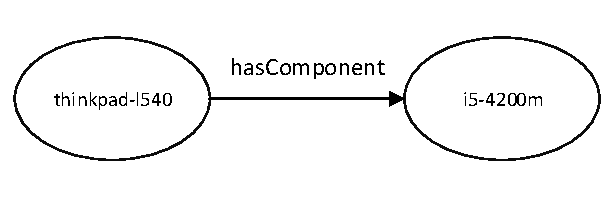
\includegraphics[height=3cm]{images/RDF-triplet.pdf}
\caption{Esimerkki kolmikosta. \label{images/RDF-triplet1}}
\end{figure}

Kaaviossa esitetään toteamus: computer hasComponent cpu. Computer on toteamuksen subjekti ja cpu on objekti. Predikaatin asemassa on "hasComponent", jonka avulla ilmaistaan, että tietokone sisältää komponentin cpu. Yhdessä edelliset toteamuksen jäsenet muodostavat kolmikon.



\subsubsection{XML/RDF}
XML/RDF on syntaksi, jonka avulla voidaan esittää RDF-tietomallin mukaista tietoa. XML/RDF syntaksi määrää tiedon esitysmuodon, jolloin tietokone ymmärtää esitetyn tiedon halutulla tavalla. Syntaksi pohjautuu XML:ään \cite{RDF_XML}. Seuraavassa on edellisen kaavion (Kuva 1) toteamus RDF/XML merkintäkielellä:

%% XML/RDF example
%% hasProduct instead of product?
\vskip 0.75cm
\begin{lstlisting}[style=codeblock]
<?xml version="1.0"?>
<rdf:RDF
xmlns:rdf="http://www.w3.org/1999/02/22-rdf-syntax-ns#"
xmlns:rel="http://www.Computer-Specs.com/semantics/relationships">

<rdf:Description
rdf:about="http://www.Computer-Specs.com/semantics/computers/example_model_001">
  <rel:hasComponent rdf:resource="http://www.Computer-Specs.com/semantics/processors/i7-8700k"/>
</rdf:Description>
</rdf:RDF>
\end{lstlisting}
\vskip 0.75cm


\begin{figure}[htb]
\centering
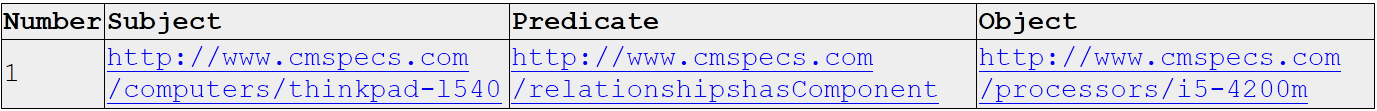
\includegraphics[width=15cm]{images/RDF-valid.PNG}
\caption{Suhteet taulukoituna. Lähde: \cite{W3C_RDF_validator}. \label{images/RDF-valid}}
\end{figure}

Ylläoleva taulukko (Kuva 2) on generoitu automaattisesti XML/RDF -merkinnän pohjalta käyttämällä W3C:n palvelua. Voimme havaita, että ulkopuolinen palvelu on ymmärtänyt esimerkkimme rakenteen oikein. Palvelu on löytänyt subjektiksi tietokoneen (example-computer), objektiksi prosessorin (i7-8700k) ja predikaatiksi "hasComponent" suhteen. Tietokoneet kykenevät siis havaitsemaan yhteyden esimerkki tietokoneen ja prosessorin välillä, kun ne lukevat edellisen XML/RDF -merkinnän.

\subsubsection{Turtle}
Nykyisin RDF:ää kirjoitettaessa suositaan paljon muitakin syntakseja kuin pelkkää XML/RDF:ää. Esimerkiksi Turtle (Terse RDF Triple Language) on tällähetkellä hyvin suosittu syntaksi sen helpon luettavuuden ja kirjoitettavuuden vuoksi \cite{cambridge2}. Turtlessa toteamukset päättyvät pisteeseen. Seuraavassa on esitetty aiempi esimerkki Turtle-syntaksilla:

%%Turle example
\vskip 0.75cm
\begin{lstlisting}[style=codeblock]
@prefix rdf: <http://www.w3.org/1999/02/22-rdf-syntax-ns#> .
@prefix rel: <http://www.Computer-Specs.com/semantics/relationships> .
@prefix computer: <http://www.Computer-Specs.com/semantics/computers> .
@prefix cpu: <http://www.Computer-Specs.com/semantics/processors> .

computer:example_model_001
  rel:hasComponent cpu:i7-8700k .

\end{lstlisting}
\vskip 0.75cm

\begin{figure}[htb]
\centering
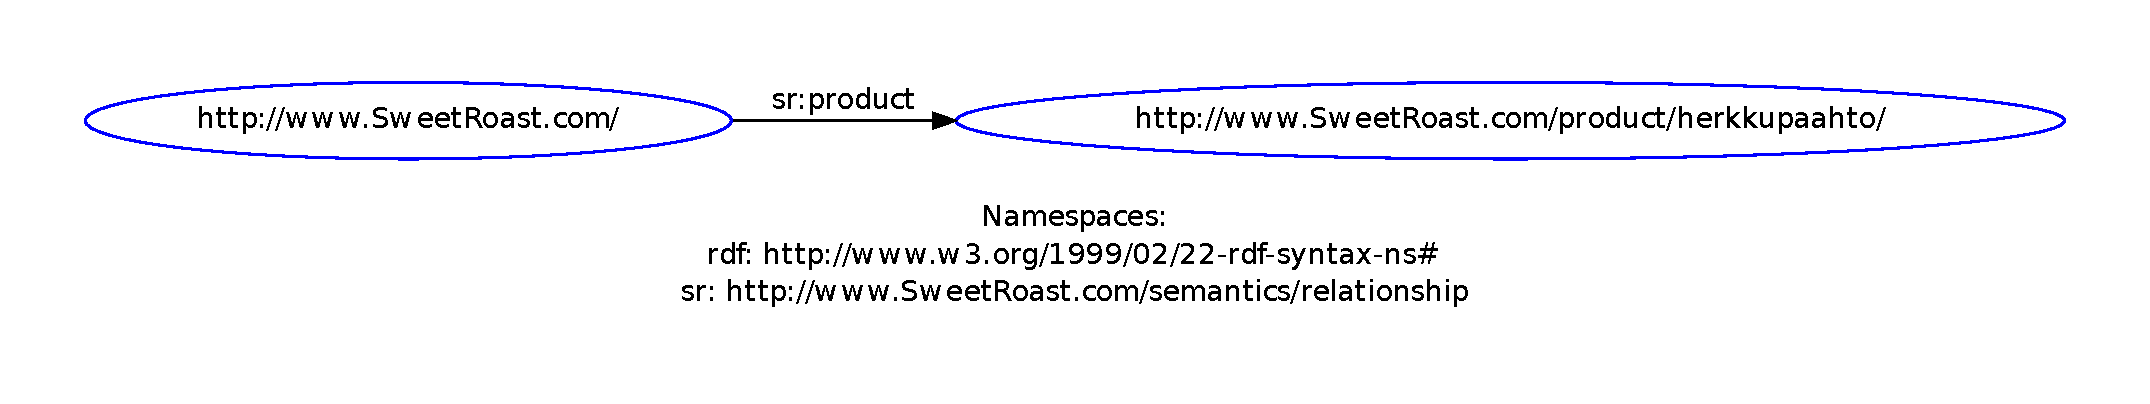
\includegraphics[width=15cm]{images/RDF-triplet2.pdf}
\caption{Turtle syntaksista automaattisesti generoitu graafi. Lähde: \cite{SeCo_RDF_validator} \label{images/RDF-triplet2}}
\end{figure}

Vaikka edelliset syntaksiin liittyvät esimerkit ovat minimaalisia, voidaan niistä kuitenkin havaita Turtle:n selkeys ja tiiveys. Turtlella RDF-lauseen kirjoittaminen ei vaadi montaa riviä tekstiä. Aluksi määritellään subjekti omalla rivillään ja sen jälkeen predikaatti ja objekti. Kolmikko päätetään aina pisteeseen.


% WHAT IS vocabulary, define
\subsubsection{Nimiavaruudet}
Etuliite eli prefiks (engl. prefix) määrää käytettävävän nimiavaruuden. Prefiksien käyttämisestä seuraa useita hyötyjä. Dokumenteista tulee siistimpiä ja helpompia lukea, koska dokumentin riveillä esiintyy vain olennista tietoa. Pitkiä URI:a ei tarvitse aina toistaa jokaisen RDF-lauseen alussa, koska tarpeelliseen URI:iin viittaaminen tapahtuu lyhyellä prefiksillä. Prefiksien käyttö nopeuttaa dokumenttien kirjoitusprosessia, koska lyhyen etuliitteen kirjoittaminen on huomattavasti nopeampaa kuin kokonaisen URI:n. Nimiavaruudet myös sallivat samannimisten termien käytön useassa eri kontekstissa, mikä on hyvin tärkeä ominaisuus.

Sama termi voi esiintyä yhdessä dokumentissa useita kertoja, mutta termillä ei välttämättä aina viitata samaan asiaan. Jotta kaksi samannimistä, mutta eria asiaa tarkoittavaa termiä voidaan erottaa toisistaan, täytyy hyödyntää nimiavaruuksia. Esimerkiksi termillä kaksipyöräinen voidaan viitata sekä polkupyörään että moottoripyörään. Mikäli halutaan yhdistää moottoriajoneuvoista- ja polkupyöristä kertovat sanastot yhdeksi kulkuneuvo sanastoksi, niin silloin termit menisivät mahdollisesti sekaisin. Voidaan kuitenkin määritellä, että etuliitteellä "mo" viitataan moottoriajoneuvoihin ja etuliitteellä "po" polkupyöriin. Näin lopullisessa kulkuneuvodokumentissa esiintyisi mo:kaksipyöräinen ja po:kaksipyöräinen, jotka tarkoittavat eri asioita.

Etuliitteet määritellään yleensä dokumenttien alussa. Esimerkiksi edellisistä syntaksiesimerkeistä voidaan havaita nimiavaruuksien määritykset ensimmäisillä riveillä. Prefiksin saa valita itse vapaasti, kunhan kyseinen etuliite ei ole jo valmiiksi käytössä. Prefiksin URI:n täytyy osoittaa olemassaolevaan resurssiin, jotta nimiavaruuden määritykset on mahdollista löytää.



\subsubsection{Semanttinen tieto}

Filosofia määrittelee termin \textbf{\textit{semantiikka}} yleiseksi teoriaksi sanojen, ilmaisujen ja lauseiden merkityksestä \cite{semantics_phi}. Tietotekniikan tutkimusala on omaksunut termin käyttöönsä, sillä termi ei määrittele tiedon esitysmuotoa, joten suomenkielisten lauseiden sijaan voidaan tutkia myös RDF-tietomallin mukaisia toteamuksia. Semantiikan näkökulmasta on mielenkiintoista, kuinka tieto voidaan esittää niin, että tiedon merkitys ymmärretään yksiselitteisesti. Semanttinen internet pyrkii erityisesti esittämään ihmiseltä peräisin olevaa tietoa niin, että tietokone ymmärtää tiedon samalla tavalla kuin ihminen \cite{Berners_visio}.

Yhtenäiset lauseet sisältävät enemmän tietoa kuin lauseenjäsenet erikseen summattuna. Esimerkiksi lauseesta "En voi ajaa tuota autoa yhdellä jalalla" ihminen voi tehdä useita päätelmiä mitä hän ei todennäköisesti tekisi yksittäisistä sanoista. Lauseesta voidaan esimerkiksi päätellä:
\begin{itemize}
  \item  Lause kertoo jostain tietystä autosta, joten ehkä lauseenkertoja osoittaa autoa.
  \item  Lauseesta käy ilmi puhujan kyvyttömyys tietyn auton ajamiseen. Ehkä auto on vääränmallinen (esim. auto on manuaalivaihteinen automaatin sijaan).
  \item  Lauseessa oleva jalka on mitä luultavimmin puhujan.
  \item  Lauseessa puhutaan yhdestä jalasta, joten ehkä puhujan jalka on hyvin kipeä tai mahdollisesti amputoitu.
\end{itemize}
Lauseiden sanajärjestyksellä on myös oma merkityksensä. Esimerkiksi lauseet "lapset söivät keksit" ja "keksit söivät lapset" eivät tarkoita samaa, vaikka ne koostuvatkin täysin samoista sanoista. Ihmiskieli siis sisältää paljon tietoa, jota on vaikea tuoda ilmi tietokoneelle \cite{semantics}.

Semanttisella tiedolla viitataan tietoon josta selviää tiedon lisäksi sen merkitys. Jotta voi ymmärtää merkityksiä, niin täytyy kyetä tunnistamaan tiedon suhteisuutta. Semanttisen internetin yhteydessä semanttisella tiedolla siis tarkoitetaan tietoa, jonka esittämiseen hyödynnetään semanttisen internetin tekniikoita. Semanttisen internetin tekniikat mahdollistavat tietokoneiden ymmärtää esitetyn tiedon lisäksi sen sisältämiä merkityksiä.

%% RDF statement -> koska lauseet sisältävät paljon tietoa!


\subsubsection{Semanttinen laadukkuus} %%poista/lyhennä? esitä tähdet/asteikko kuvana?
Semanttisen tiedon määrittäminen vaatii aihealueen asiantutemusta ja runsaasti kehitystyötä, minkä vuoksi osa jaetusta tiedosta on laadukkaampaa kuin muu. Tästä syystä Tim Berners-Lee on luonut asteikon, jonka avulla tarjolla olevaa linkittynyttä tietoa voidaan luokitella. Berners-Leen esittelemä asteikko arvostelee tietolähteen 1-5 tähdellä. Yhden tähden saa sillä, että tieto on vapaasti jaossa internetissä. Kaksi tähteä saa, jos tieto on tietokoneen luettavissa. Kolme tähteä ansaitsee, kun tietokoneluettava tieto esitetään yleisesti käytettävissä olveassa standardoidussa muodossa. Kun tarjolla oleva tieto noudattaa RDF-tietomuotoa, niin silloin on mahdollista ansaita neljä tähteä. Viiteen tähteen vaaditaan kaikki edellämainitut kohdat, sekä tiedon tulee olla myös linkitettyä muuhun ulkopuoliseen tietoon \cite{Tim-BL}. Arvosteluasteikkoa on ehdotettu laajennettavaksi välille 1-7 tähteä SeCo:n (Semantic Computing Research Group) toimesta \cite{SeCo_stars}. He esittävät, että tieto on kuuden tähden arvoista, jos tietoa kuvaavat skeemat on kuvailtu eksplisiittisesti ja ne on mahdollista saada tiedon yhteydessä. Seitsemään tähteen vaadittaisiin tiedon ja skeemojen erillistä tulkintaa, jolla varmistettaisiin, että tieto ja skeemat liittyvät selkeästi toisiinsa. Näin ulkopuolinen tietoa hyödyntävä taho voisi varmistua tiedon laadukkuudesta ja soveltuvuudesta jatkokäyttöä varten. Tällähetkellä ongelmana on se, että ulkopuolinen taho ei voi nopeasti tietää mikäli sanasto on laadukas. Sanastoon täytyy ensin tutustua, jotta voidaan tehdä päätelmiä sen soveltuvuudesta ja laadukkuudesta. Esitetyn arvosteluasteikon on tarkoituksena ratkaista edellinen ongelma.

//Check Publishing on the ... source

\subsection{RDF Schema}
%%Usein tietoa halutaan kuvata tarkasti, jolloin RDF:n tukena tulee käyttää RDF Schemaa.
RDF Schema (Resource Description Framework Schema) mahdollistaa tietojoukkojen ja toisiinsa liittyvien resurssien kuvailun. RDFS tarjoaa RDF:n jatkeena lisämahdollisuuksia tiedon kuvailemiseen. Esimerkiksi luokkamäärittelyt ovat yksi erittäin tärkeä RDFS:n työkalu, minkä avulla voidaan kuivalla ryhmittynyttä tietoa \cite{W3C_RDFS2}. RDFS:n avulla voidaan siis kuvailla yleisellä tasolla esimerkiksi talon ominaisuuksia, kun taas RDF:llä voidaan kuvata ainoastaan yksittäisen tunnetun talon ominaisuuksia \cite{Antoniou}. RDF Schema on kirjoitettu RDF:n avulla, joten RDFS:ää hyödyntävät tiedostot ovat myös valideja RDF-graafeja. \cite{RDF_specification_old}

Luokkien määrittäminen auttaa järjellisen tiedon esittämisessä. Luokan avulla voidaan luoda rajoitteita liittyen RDF väitteisiin, mikä estää mielettömät väitteet. Voimme esimerkiksi määritellä kirjoittaja ominaisuuden, joka kuuluu ainoastaan kirjaluokalle. Tämän jälkeen voidaan järjellisesti todeta, että kirjan Viilipytty kirjoittaja on Matti. Luokan määrittely kuitenkin estää esittämästä järjettömiä väitteitä, kuten esimerkiksi "Helsingin kirjoittaja on Matti" \cite{Antoniou}.

Scheman luokat muistuttavat luokkapainotteisten ohjelmointielten luokkia. Selvänä erona on kuitenkin tapa jolla luokan ominaisuudet määritetään. Tavallinen ohjelmointikieli voi määrittää esimerkiksi luokan \textit{auto} koostuvan renkaista, ovista ja moottorista. Kun luokasta luodaan autoinstanssi, niin sillä on aina edelliset ominaisuudet. \textcolor{red} {RDF Schemassa luokan ominaisuudet kuvataan resurssikohtaisesti} \cite{W3C_RDFS2}. Tämän vuoksi kaikki luokan instanssit eivät välttämättä omaa täysin samoja ominaisuuksia. RDFS:n tapa sallii luokkamääritelmien tarkentamisen ja jatkamisen ilman mahdollisuutta muokata alkuperäistä kuvausta. Tämä sallii käyttäjien jatkaa toisten tekemiä määritelmiä omaan käyttöön sopivaksi.

Tärkeitä RDFS:n ominaisuuksia ovat muun muassa \textit{domain}, \textit{range} ja \textit{subClassOf}, mitkä liittyvät vahavasti luokkiin. Domainin avulla voidaan määrittää tietyn ominaisuuden kuuluvan tietylle luokalle. Voidaan esimerkiksi määrittää autoluokka ja predikatti "hasMotor". Domainin avulla voimme kertoa, että hasMotor-predikaatti kuuluu autoluokalle, joten predikaattia on mieletöntä käyttää kuvailemaan esimerkiksi auton rengasta. Rangen avulla määritetään mihin predikaatilla voidaan viitata. Edellisen esimerkin tapauksessa olisi järkevää määrittää "hasMotor" predikaatin rangeksi moottoriluokka. Siten auton moottori voi olla ainoastaan moottoriluokan ilmentymä eikä esimerkiksi "korkea". RDFS:n "subClassOf" ominaisuuden avulla voidaan esitellä alaluokkia, mikä mahdollistaa luokkahierarkioiden kuvaamisen. Autoluokan alaluokka voisi olla esimerkiksi farmari.

Seuraavassa on Turtle-syntaksilla kirjoitettu esimerkki edellä esitellyistä RDF Scheman ominaisuuksista. Esimerkissä määritetään aluksi akku, tietokone ja kannettava tietokone luokat. Kannettava tietokone on tietokoneen alaluokka. Seuraavaksi määritellään "hasBattery" ominaisuus, minkä avulla voidaan kuvata, että kannettava tietokone sisältää akun. Lopuksi luodaan akusta ja kannettavasta tietokoneesta ilmentymät. Kannettava tietokone sisältää edellä määritetyn akun. Esimerkissä hyödynnetään Turtlen ominaisuutta lyhentää toteamuksia määrittelemällä toteamusten subjekti ainoastaan kerran. Puolipisteen jälkeiset toteamukset viittaavat edelleen samaan subjektiin, kun taas pisteen jälkeen määritetään aina uusi subjekti.

%% RDFS
\vskip 0.75cm
\begin{lstlisting}[style=codeblock]
@prefix ex: <http://www.Computer-Specs.com/semantics/example> .
@prefix rdf: <http://www.w3.org/1999/02/22-rdf-syntax-ns#> .
@prefix rdfs: <http://www.w3.org/2000/01/rdf-schema#> .
@prefix xsd: <http://www.w3.org/2001/XMLSchema#> .

# Class definitions
ex:Battery  rdf:type rdfs:Class .
ex:Computer rdf:type rdfs:Class .
ex:Laptop   rdf:type rdfs:Class ;
    rdfs:subClassOf ex:Computer .

# Data properties
ex:hasBattery a rdf:Property ;
    rdfs:domain ex:Laptop ;
    rdfs:range  ex:Battery .

# Instances
ex:4X50M33573 a ex:Battery ;
    ex:hasPower "32"^^xsd:integer ;
    ex:hasVoltage "15.4"^^xsd:float .

ex:ThinkPad_E570 a ex:Laptop ;
    ex:hasBattery ex:4X50M33573 .


\end{lstlisting}
\vskip 0.75cm

\begin{figure}[htb]
\centering

%% huomaa kuinka läppärin ominaisuudet kerrotaan vasta instanssissa eikä luokkamäärityksissä.
%% huomaa kuinka toteamukset voivat loppua pisteeseen tai puolipisteeseen.

%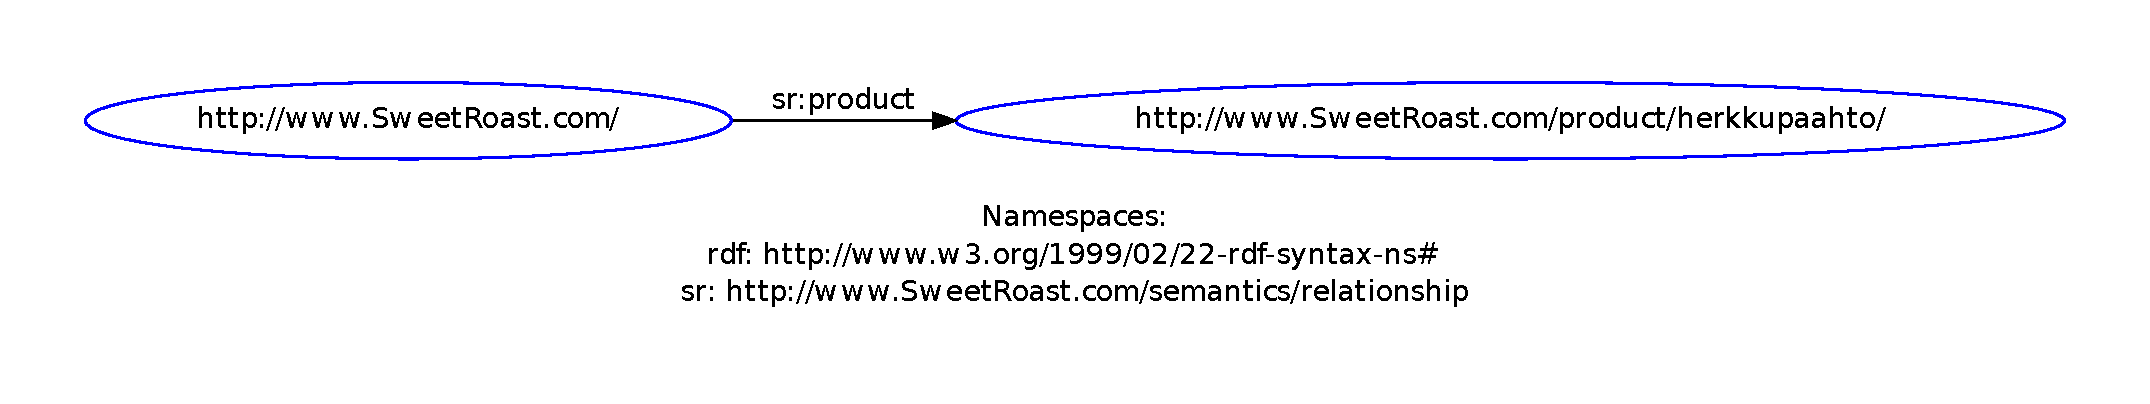
\includegraphics[width=15cm]{images/RDF-triplet2.pdf}
%\caption{Turtle syntaksista automaattisesti generoitu graafi. Lähde: \cite{SeCo_RDF_validator} \label{images/RDF-triplet2}}
\end{figure}
%% Lisää viittaus??: https://www.youtube.com/playlist?list=PLea0WJq13cnDDe8V7eVLReIaOnFztOEAq
\subsubsection{Ontologiat ja sanastot}
%% Littyy rdfs
Sanastolla (engl. vocabulary) tarkoitetaan määritelmiä, joiden avulla tietoa voidaan kuvata sovellustarkoitukseen sopivassa muodossa \cite{RDF_specification}. Sanastoja hyödynnetään tiedon integroinnissa ja organisoinnissa \cite{vocabulary}. Esimerkiksi tuotteen maahantuojan tuotetietojen ja kauppiaan myyntitetojen yhdistäminen voi olla hyödyllistä. Kauppiaan ei tarvitse kuvailla myymien tuotteidensa ominaisuuksia, koska hän voi hyödyntää maahantuojan valmiita kuvauksia. Kauppias ja myyjä eivät kuitenkaan todennäköisesti kuvaile tuotetteita täysin samalla RDF-termistöllä. Siksi tarvitaan sanasto, jonka avulla voidaan esittää tarpeellinen lisätieto. Ilman sanastoa tietokone ei kykene yhdistämään maahantuojan tuotekuvausta ja myyjän vastaavaa tuottetta toisiinsa.

Sanastoja kirjoitetaan RDF Scheman avulla. Sanastoilla voidaan määrittellä sovellukselle ominaisia tiedon rakenteita ja rajoitteita. \cite{vocabulary}. Esimerkiksi rakennussovellusta varten voitaisiin määrittellä "yhteensopiva" predikaatti, sekä erilaisia mutteri ja pultti resursseja. Tämän jälkeen voitaisiin määritellä, että saman kierteen omaavat pultit ja mutterit ovat yhteensopivia, minkä seurauksena sovelluksen käyttöliittymä voisi tarjota käyttäjälle ainoastaan yhteensopivia rakennustarvikevaihtoehtoja. Sanastoja on paljon erilaisia ja niitä voi tarvittaessa luoda lisää \cite{RDF_specification}. Hyvin määriteltyjä sanastoja voidaan uudelleenkäyttää ja jakaa muiden kesken. Esimerkiksi Dublin Core ja Friend of a Friend (FOAF) ovat hyvin tunnettuja ja maailmanlaajuisesti RDF:n yhteydessä käytettyjä sanastoja \cite{data_namespace}.

Ontologiat ovat kokoelmia toteamuksista, jotka määräävät konseptien välisiä suhteita ja määrittelevät loogisia sääntöjä, joiden avulla tietoa voidaan järkeillä \cite{Berners_visio}.
Siten ontologiat ovat kuin metadataskeemoja, jotka määrittelevät konseptien esittämiseen käytettävän sanaston. Kun konseptit määritellään eksplisiittisesti ja niiden semantiikka ilmaistaan koneluettavassa muodossa, niin ontologiat tehostavat ihmisen ja tietokoneen välistä kommunikointia \cite{ontology_learning}. Ontologioiden ero sanastoihin on niiden monimutkaisempi ja formaalimpi rakenne. Toisinaan ontologioita ja sanastoja voi olla vaikea erottaa toisistaan, joten termejä voidaan käyttää myös toistensa synonyymeinä \cite{vocabulary}.

Ontologioiden luominen vaatii sovelluskohteen asiantuntemusta ja kehitystyötä.
Kehitykseen kuluvaa aikaa voidaan vähentää hyödyntämällä erilaisia ohjelmistoja, jotka ovat erikoistuneet ontologioiden luomiseen. Ohjelmistoilla ei voida kuitenkaan korvata asiantutemusta, sillä kehittäjän täytyy tuntea kuvailtava tieto, jotta hän voi luoda siihen liittyviä sääntöjä. Esimerkiksi onnistuneen luokkajaottelun tekeminen on hyvin vaativaa, mikäli kehittäjä ei hahmota kuvailtavan tiedon suhteita. Lisäksi kehittällä tulee olla tietämystä semanttisen internetin tekniikoista, jotta hän osaa käyttää niitä. Ontologioiden luomiseen käytetään RDF Schemaa ja OWL-tietämyksenesttämiskieltä \cite{OWL_specification}.



\subsection{OWL}

OWL (Web Ontology Language) on semanttisen internetin yhteydessä käytetty tietämyksenesttämiskieli. Tietämyksenesittämiskielille tärkeitä ominaisuuksia ovat selkeästi määritelty syntaksi, formaali semantiikka, riittävä ilmaisuvoima ja päättelytuki \cite{Antoniou}. Käyttötarkoitukseltaan OWL on rinnastettavissa RDF Schemaan, mutta ilmaisuvoimaltaan OWL on huomattavasti tehokkaampi kuin RDFS. RDF Schema tarjoaa ainoastaan vähimmäisedellytykset semanttisen tiedon kuvaamiseen \cite{revisited}. Ilmaisuvoimaisen OWL:n avulla voidaan luoda ontologioita \cite{OWL_specification}.

Formaalilla semantiikalla tarkoitetaan kykyä ilmaista esitetyn tiedon merkitys tarkasti ja yksiselitteisesti \cite{Antoniou}. Tämä mahdollistaa päättelyn esitetyn tiedon pohjalta. Esimerkiksi alaluokkasuhde mahdollistaa yksinkertaisen päättelyn, sillä joutsenluokkaan kuuluva laulujoutsen kuuluu selvästi myös lintuluokkaan. Edellinen päätelmä voi olla tarpeellinen esimerkiksi sovelluksessa, joka listaa kaikki Suomen sorsaeläimet, kun tarkastellaan laulujoutsenta. OWL tarjoaa useita keinoja pääteltävän tiedon määrittelyyn, mikä tekee siitä ilmaisuvoimaisen.

Owl määrittelee muun muassa funktionaalisen, transitiivisen ja symmetrisen luokkaominaisuuden. Edelliset ominaisuudet eivät ole ainoita OWL:n ominaisuuksia, mutta niiden tarkoitus on antaa lukijalle riittävä mielikuva OWL:n tarjoamista mahdollisuuksista määritellä tietoa. Funktionaalisella ominaisuudella tarkoitetaan instanssien välistä suhdetta, jossa instanssia kohden voi ilmetä ainoastaan yksi uniikki arvo. Esimerkiksi auton ja rekisterinumeron välistä suhdetta voidaan kuvata funktionaalisella ominaisuudella. Transitiivisella ominaisuudella voidaan kuvata pääteltäviä osakokonaisuus suhteita. Esimerkiksi pöydänjalan ollessa pöydän osa ja ruuvin ollessa pöydänjalan osa, voidaan päätellä, että ruuvi on myös pöydän osa. Symmetrisellä ominaisuudella viitataan ystävyyssuhdetta vastaavaan ilmentymään. Yleensä ystävät kokevat toisensa ystävikseen, joten suhde on molemminpuoleinen eli symmetrinen \cite{OWL_specification}.


%OWL-tietämyksenesttämiskielestä on kolme erilaista versiota: OWL Full, OWL DL ja OWL Lite. Kielien ero on niiden laajuudessa ja kyvyssä kuvata tietoa. OWL Full on kaikista laajin ja se on RDFS yhteensopiva \cite{OWL_specification}.

Seuraavassa on esitetty RDF Schema osion kannettava tietokone esimerkki täydennettynä OWL:lla. Esimerkistä voidaan huomata, että se näyttää edelleen hyvin samalta kuin aiemmin. OWL-määritelmät ovat lisätietoa. Esimerkin Turtle-merkintä on generoitu protégé nimisellä ohjelmistolla, jonka avulla voidaan tuottaa ontologioita tehokkaasti \cite{Protege}.

%%
\vskip 0.75cm
\begin{lstlisting}[style=codeblock]
@prefix : <http://www.Computer-Specs.com/ontologies/example#> .
@prefix owl: <http://www.w3.org/2002/07/owl#> .
@prefix xml: <http://www.w3.org/XML/1998/namespace> .
@prefix xsd: <http://www.w3.org/2001/XMLSchema#> .
@prefix rdf: <http://www.w3.org/1999/02/22-rdf-syntax-ns#> .
@prefix rdfs: <http://www.w3.org/2000/01/rdf-schema#> .
@base <http://www.Computer-Specs.com/ontologies/example> .

<http://www.Computer-Specs.com/ontologies/example> rdf:type owl:Ontology .

# Object Properties
:hasBattery rdf:type owl:ObjectProperty ;
            rdfs:domain :Laptop ;
            rdfs:range :Battery .

# Data properties
:hasPower rdf:type owl:DatatypeProperty ;
          rdfs:domain :Battery .

:hasVoltage rdf:type owl:DatatypeProperty ;
            rdfs:subPropertyOf owl:topDataProperty ;
            rdfs:domain :Battery .

# Classes
:Battery  rdf:type owl:Class .
:Computer rdf:type owl:Class .
:Laptop   rdf:type owl:Class ;
          rdfs:subClassOf :Computer .

# Individuals
:C52863 rdf:type owl:NamedIndividual ;
        :hasPower "57"^^xsd:int ;
        :hasVoltage "10.8"^^xsd:float .

:ThinkPad_T570 rdf:type owl:NamedIndividual ,
                           :Laptop ;
               :hasBattery :C52863 .

\end{lstlisting}
\vskip 0.75cm


\subsection{RDF tiedon säilöminen}


\subsubsection{Triple store}
RDF-tietomuodossa olevaa tietoa voidaan tallentaa muistiin. Yksinkertaisimillaan voidaan tallentaa suoraan RDF/XML, Turtle tai vastaavia tiedostoja, mutta tämä ei ole kovin tehokasta. Yksittäisen tarpeellisen asian etsiminen on hidasta, kun tiedostokoot ovat suuria. Tästä syystä on kehitetty tehokkaampiakin tallennustapoja, jotka hyödyntävät tietokantoja. Triple store on tietokantatyyppi, joka on suunniteltu erityisesti RDF-graafien tallentamiseen. RDF-tieto on todella linkittynyttä, minkä vuoksi graafi-tietokannat soveltuvan sen tallentamiseen paremmin kuin perinteiset relaatiotietokannat. Relaatiotietokannoissa useiden linkittyneiden asioiden välille on huomattavasti vaikeampaa luoda suhderakenteita ja kyselyiden tekeminen on myös haastavaa. Triple store tietokanta tallentaa RDF lauseet suoraan kolmikkoina, joten sovelluskohtaisia relaatiotauluja ei tarvitse luoda \cite{triplestore}. Tarkka standardointi sallii tiedon hakemisen myös ulkopuolisista avoimista tietokannoista. Tämän ansiosta tietokantoja voidaan linkittää, mikä mahdollistaa tavallista laajemman tiedonhaun.

\begin{figure}[htb]
\centering
\includegraphics[width=15cm]{images/linked_data.png}
\caption{Graafi vapaasti hyödynnettävistä linkittyneistä tietokannoista vuonna 2017. (LOD cloud diagram) \cite{LOD_cloud} \label{images/linked_data}}
\end{figure}
\clearpage

\subsubsection{SPARQL}

SPARQL on spesifikaatiokokonaisuus, joka tarjoaa kieliä ja protokollia RDF-graafien muokkaamiseen ja kyselyiden tekemiseen \cite{sparql}. SPARQL ei ole yksittäinen kieli, vaan se koostuu useita hyödyllisistä ja tarpeellisista osista. Tässä alaluvussa keskitytään ainoastaan SPARQL Query Languagen perusteisiin.

SPARQL Query Languagen avulla voidaan hakea RDF-muotoista tietoa triple store tietokannoista. Jokaisella triple storella on \textcolor{red}{päätepiste} (engl. endpoint), johon SPARQL kyselyt voidaan lähettää HTTP (Hypertext Transfer Protocol) protokollan avulla. Päätepisteen luominen internettiin on helppoa, joten avoimia päätepisteitä on paljon tarjolla. Esimerkiksi dbpedia tarjoaa avoimen päätepisteen (http://dbpedia.org/sparql), josta voi hakea tietoa RDF-tietomuotoisesta Wikipediasta \cite{Antoniou}.

RDF:ssa toteamukset koostuvat subjektista, predikaatista ja objektista. SPARQL kyselylauseessa jokin edellisistä RDF-toteamuksen osista voidaan korvata muuttujalla, mitä merkitään kysymysmerkillä \cite{Antoniou}. SPARQL etsii kyselylausetta vastaavat toteamukset ja palauttaa niistä muuttujan paikalle sopivat arvot. Kyselylause voi olla esimerkiksi seuraavanlainen:

\begin{lstlisting}[style=codeblock]
PREFIX ex: <http://www.Computer-Specs.com/ontologies/example#> .

SELECT ?battery
WHERE {
  ex:ThinkPad_T570 ex:hasBattery ?.
}
\end{lstlisting}

Koska ThinkPad\_T570:n akuksi on aiemmissa luvuissa määritelty "C52863", niin SPARQL palauttaa käyttäjälle kyseisen akun. Kyselyn tulos voi koostua myös useammasta kuin yhdestä arvosta, mikäli useampi toteamus toteuttaa kyselyn. Jotta SPARQL tietää mistä se etsii tietoa, niin sille täytyy kertoa kyselyn nimiavaruudet prefiksien avulla.

SPARQL tarjoaa monia keinoja hakujen tekemiseen. Kyselyssä voi esiintyä useita muuttujia.
Haut voivat koostua liitoksista (engl. union) ja negaatioista. Lukuarvoista koostuva tulos voidaan summata yhteen sum-funktion avulla. Tulokset voidaan myös järjestellä haluttuun järjestykseen "ORDER BY" lauseen avulla. Haku voi myös olla SELECT kyselyn sijaan ASK-tyyppinen, joka testaa mikäli haulla on olemassaolevia ratkaisuja ja palauttaa tuloksen mukaisen boolean arvon \cite{sparql_query}. SPARQL tarjoaa useita erilaisia syntakseja kyseltuloksen esittämiseen. Kyselyn tulos voidaan esimerkiksi esittää Turtle tai XML/RDF syntaksin mukaisessa muodossa. \cite{W3C_turtle}.

Syntaksiltaan SPARQL muistuttaa SQL kyselykieltä.


\clearpage
%%===============================================================================

\subsection{Linkittynyt tieto}

\clearpage
%%===============================================================================
\section{Käytännönsoveltuvuus}
Esimerkiksi Facebook käyttää semanttista verkkoa tiedonhaussa, minkä avulla se kykenee tarjoamaan käyttäjilleen parempia hakutuloksia \cite{Facebook}.

Hakukoneoptimointi -> nettisivujen löydettävyys.
https://www.profium.com/en/blog/semantic-search-in-employment-matching
Semantic search in emplyment matchin.
Työhakemusten lukemisessa käytetään paljon automattisia ohjelmistoja, jotka yrittävät löytää kaikista sopivimmat hakijat [lähde...]. Tämä säästää yritysten aikaa ja rahaa, koska soveltumattomiin hakijoihin ei tarvitse käyttää resursseja. Ongelmallista tässä tavassa on kuitenkin se, että se voi jättää hyviä hakijoita havaitsematta ja soveltumattomien ehdokkaiden on mahdollista tulla havaituksi, mikäli he tuntevat käytetyn järjestelmän. Järjestelmät tyypillisesti etsivät muun muassa määriteltyjä avainsanoja hakemuksista [lähde]. Jos työhakemus ei ole koneluettava (esimerkiksi kuvaskannaus työhakemuksesta), niin silloin järjestelmät eivät voi löytää avainsanoja, jolloin hakemus todennäköisesti hylätään.

Semanttinen työnhaku m


\subsection{XMP-metadataformaatti}
\subsection{Finlex}

\clearpage
%%===============================================================================
\section{Semanttisen verkon nykytila ja tulevaisuus}
%%kerro haasteista, tilasta, tulevaisuudesta
%% haasteita: yksityisyys, tiedon jaon halukkuus, ylimääräinen työ ontologioiden esiottämisessä kielien jäykkyys.
%% RDF ongelmia:
%% http://milicicvuk.com/blog/2011/07/21/problems-of-the-rdf-syntax/

%% Semantic web revisited - loppu ontologioiden kehitystyö ja hinta
%% Amazon neptune - RDF database
%% Google knowledge graph

%% hyöty: dissertio p.28 "service discovery" - yhteinen kieli

%% katso lähde WWW: Past..

%% LOD-graafi. Käyttökohteita: Life sciences, Government, Linguistic, Social network, Publications.

Semanttinen internet ei tarkoita tekoälyä. Siten ei ole tekoälyä, joka tekee omia päätelmiä dokumenteista, vaan ihmisen tulee itse kirjoittaa semanttisia dokumentteja \cite{Semantic_Web_represent}. Semanttinen tieto näyttää samalta kuin tavallinen teksti, minkä vuoksi moni voi olla haluton käyttämään enempää aikaa semantiikan määrittämiseen.

\subsection{Semanttisen internetin arkkitehtuuri}
Tietotekniikan yhteydessä arkkitehtuurilla viitataan ratkaisujen jäsentelyyn eli rakenteeseen. Semanttinen internet koostuu selkeistä komponenteista, joten voidaan puhua, että semanttisella internetillä on oma arkkitehtuurinsa. Tim-Berners lee esitteli vuonna 2000 semanttisen internetin arkkitehtuurin seuraavanlaisena:

\begin{figure}[htb]
\centering
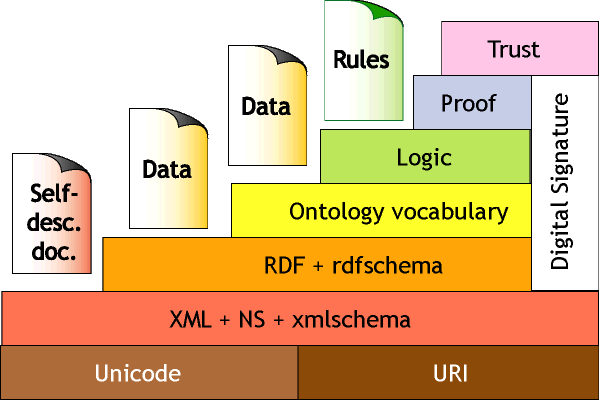
\includegraphics[width=10cm]{images/sweb-stack.png}
\caption{Tim Berners-Leen esittämä pinomalli. Lähde: \cite{stack_bl} \label{images/sweb-stack.png}}
\end{figure}
\clearpage %% Force images on same paragraph

Semanttinen internet kehittyy jatkuvasti. Toisinaan syntyy uusia tarpeita, jolloin kehitetään uusia tekniikoita, mitkä saattavat korvata vanhentuneita tekniikoita. Tästä syystä semanttisen internetin arkkitehtuuri on jatkuvasti altis muutoksille. Vuoden 2000 arkkitehtuuri ei päde enään tänäpäivänä.

Vastaavanlainen ilmiö voidaan myös havaita internetin kohdalla tekniikoiden kehittymisenä, vanhentumisena ja vaihtumisena.

\begin{figure}[htb]
\centering
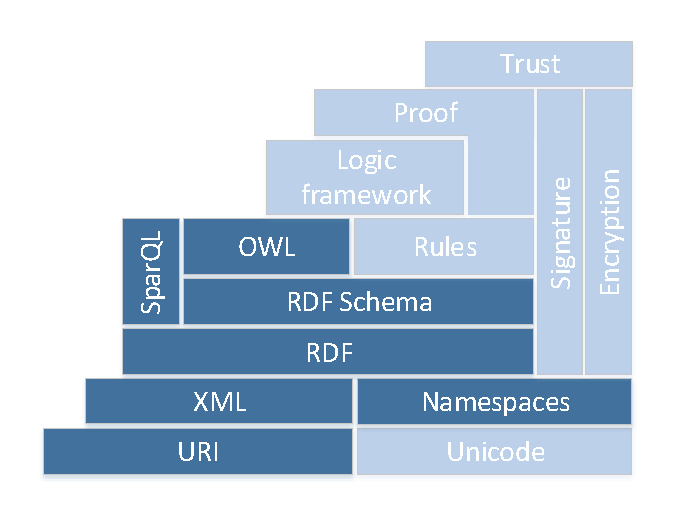
\includegraphics[width=10cm]{images/sweb-stack2.pdf}
\caption{Vuonna 2005 esitetty arkkitehtuuri. \label{images/sweb-stack2.pdf}}
\end{figure}


Ylläolevan kuvan pino noudattaa NNN:n johtamaa mallia \cite{stack}. Kuvasta on himmennetty aiheet joita ei ole käsitelty tässä työssä. Semanttisen internetin pino muistuttaa edelleen jälkimmäistä pinoa. W3C ei ole julkaissut uusia semanttisen internetin standardeja ja se onkin päätynyt päivittämään aiempia standardeja viime vuosina.


\clearpage %% Force images on same paragraph

\subsection{haasteet}
Semanttinen verkko ei tarjoa ratkaisua yksittäiseen ongelmaan, joten semanttisen verkon markkinointi on haastavaa. Sovellusten kehitys ei ole myöskään aivan suoraviivaista, mikäli niiden halutaan hyödyntävän semanttista internettiä täydessä potentiaalissaan \cite{lassila_dissertion}.

\subsection{kehitys}
Goel et al. on kerännyt statistiikkaa liittyen semanttiseen merkintään. Statistiikka on saatu keräämällä satunnainen näyte miljoonasta web sivusta. Kesäkuussa 2010 \cite{Google} (s.3). Semanttikkaa (Microformats tai RDFa) käytti ainoastaan 42 605 sivua eli alle puoli prosenttia. Vuonna 2010 semanttisen materiaalin osuus on ollut siis olematon.

\clearpage
%%==============================================================================
\section{Yhteenveto}



\clearpage
%%==============================================================================
\section{Text dump (temporary)}

Jotta tietokoneet kykenevät tekemään loogisia päätelmiä tiedosta, niin tieto täytyy esittää sopivassa muodossa.

Tietokoneiden ymmärrettävissä oleva tieto on erittäin arvokasta. Tietokoneet voivat tehdä itsenäisiä loogisia päätelmiä ja löytää uusia asiayhteyksiä, joiden esittämisestä saattaa olla hyötyä käyttäjälle. Tietokoneiden ei tarvitse olla ainoastaan ihmisen työkaluja, vaan ne voivat olla myös apureita. Tiedon ymmärtäminen ei kuitenkaan tarkoita yksittäisten sanojen löytämistä, vaan asiayhteyksien havaitsemista tiedonpalasten välillä. Jotta tietokone kykenee havaitsemaan asiayhteyksiä, niin tie



Tietokoneet eivät ymmärrä tiedon välisiä suhteita suoraan tekstistä kuten ihmiset. Sanat ja lauseet eivät itsessään tarkoita tietokoneelle mitään. Sanat koostuvat erilaisista kirjainyhdistelmistä, jotka voidaan esittää binääreinä \cite{ASCII}. Sanojen välille ei kuitenkaan voida suoraan luoda asiayhteyksiä. Tietokone ei esimerkiksi kykene tunnistamaan synonyymejä terveyskeskus ja terveysasema, vaan tietokone käsittää ne täysin erillisinä sanoina. Tästä syystä tarvitaan lisätietoa, jonka avulla tietokoneelle voidaan kertoa sanojen merkitys ja suhde.

\clearpage
%%==============================================================================
%% Lähdeluettelo - toisesta tiedostosta
\bibliographystyle{acm}
\bibliography{bibliography.bib}
\clearpage
%%==============================================================================
\thesisappendix

\section{Syntaksi esimerkit\label{LiiteA}}

Tässä liitteessä on esitelty yhtenäisiä esimerkkejä kahviyhtiö SweetRoast Co:sta ja sen tuotteista. Tekstin sekaan upotetuista lyhyistä näytteestä voi olla hankalaa hahmottaa kielten syntaksia, joten laajemmat esimerkit ovat tarpeen. Tekstin seassa olevat lyhyet esimerkit ovat kuitenkin myös tarpeellisia, sillä niiden tarkoitus on toimia apuvälineenä esitetyn asian ymmärtämisessä. Seuraavat esimerkit siis laajentavat jo aiemmin esitettyjä esimerkkejä. (TODO: viimeistele esimerkit, validoi ja lisää graafit)

Esimerkiksi pöytätietokoneen rakenne voidaan kuvata seuraavasti XML-merkintäkielen avulla:
\subsection{XML esimerkki}
\lstinputlisting[style=codeblock]{files/full_xml.txt}
\vskip 0.75cm

\subsection{XML/RDF esimerkki}
\lstinputlisting[style=codeblock]{files/full_rdf.txt}

\begin{figure}[htb]
\centering
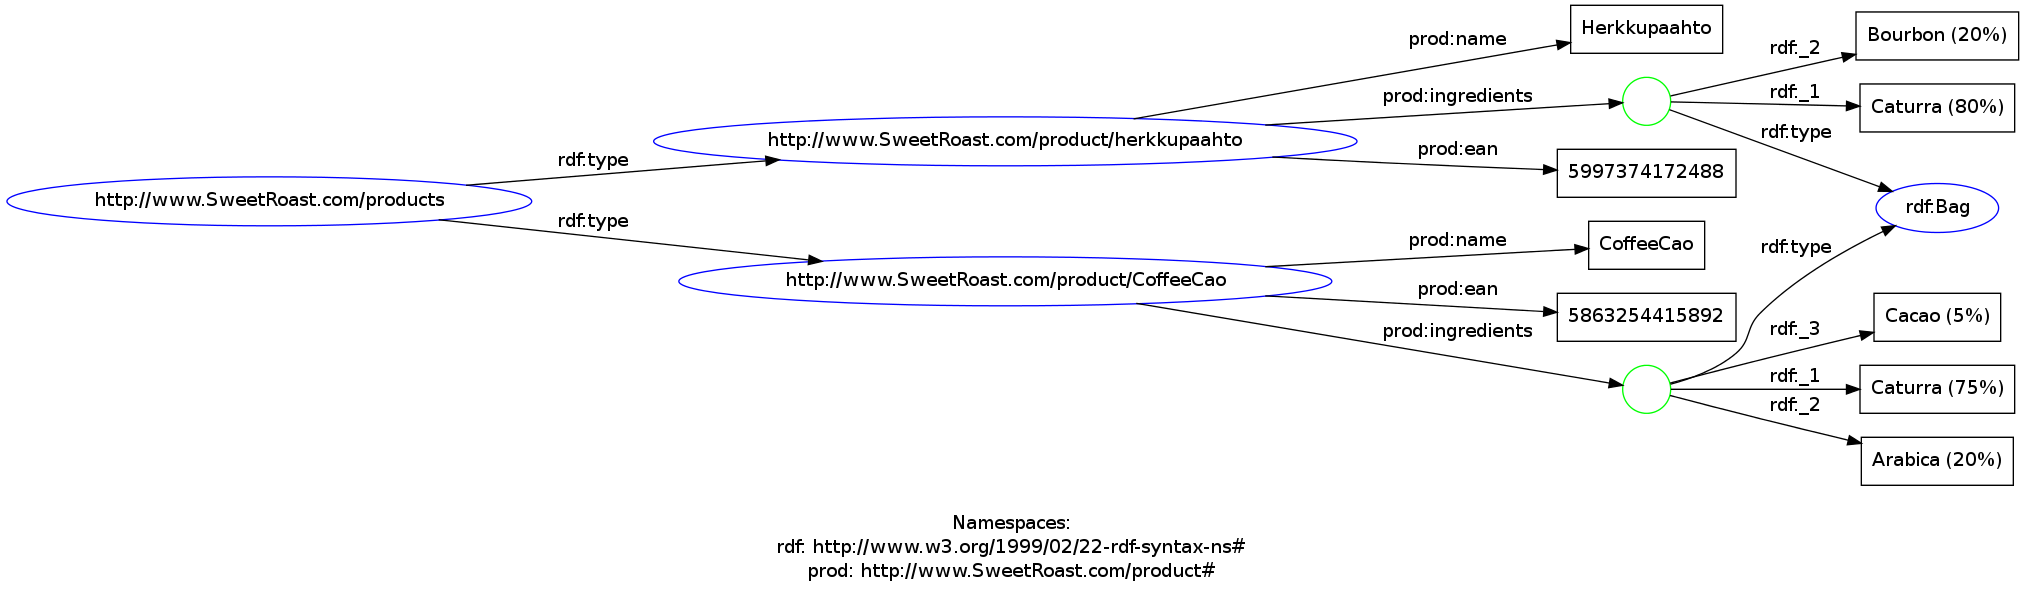
\includegraphics[width=15cm]{images/xml-rdf-seco.png}
\caption{Automaattisti generoitu graafi ylläolevasta merkinnästä. Lähde:\cite{SeCo_RDF_validator} \label{images/xml-rdf-seco.png}}
\end{figure}
\vskip 0.75cm
\clearpage

\subsection{Turtle esimerkki}
\lstinputlisting[style=codeblock]{files/full_turtle.txt}
\vskip 0.75cm



\end{document}
